\section{Fast poisson logpmf}
\subsection{The implementations}
The poisson logpmf is something aaaa

We have four different implementations performing (poisson logpmf?) ... :


\definecolor{keywordclr}{rgb}{0,0,1}
\definecolor{stringclr}{rgb}{0.75,0.15,0.15}
\definecolor{commentclr}{rgb}{0.5,0.5,0.5}

\lstset{frame=tb,
  language=Python,
  aboveskip=3mm,
  belowskip=3mm,
  showstringspaces=false,
  columns=flexible,
  basicstyle={\small\ttfamily},
  numbers=left,
  numberstyle=\smaller\color{commentclr},
  keywordstyle=\color{keywordclr},
  commentstyle=\color{commentclr},
  stringstyle=\color{stringclr},
  breaklines=true,
  breakatwhitespace=true,
  tabsize=4
}

The first implementation we consider is the implementation provided by the SciPy \cite{SciPy}
\begin{lstlisting}
from scipy.stats import poisson

def poisson_logpmf(k, r):
    return poisson.logpmf(k, r)
\end{lstlisting}

\pgfplotsset{
  compat=newest,
  xlabel near ticks,
  ylabel near ticks
}

\begin{figure}[ht!]\label{figure:poisson_logpmf_performance}
\begin{center}
  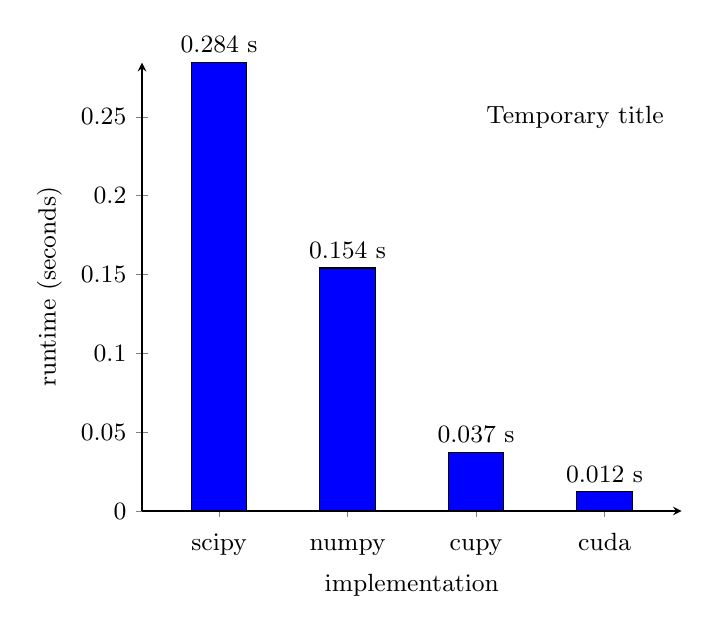
\begin{tikzpicture}[font=\small]

  \node at(5.5,5)(title){Temporary title};
 
\

\begin{axis} [
  ylabel={runtime (seconds)},
  xlabel={implementation},
  ybar,
  bar width=20pt,
  ymin=0,
  %ytick=\empty,
  xtick=data,
  axis x line=bottom,
  axis y line=left,
  enlarge x limits=0.2,
  symbolic x coords={scipy, numpy, cupy, cuda},
  xticklabel style={anchor=base, yshift=-\baselineskip},
  /pgf/number format/.cd,fixed,precision=3,
  nodes near coords={\pgfmathprintnumber{\pgfplotspointmeta} s},
]

\addplot[fill=blue] coordinates {
    (scipy, 0.2843504619598389)
    (numpy, 0.15413585186004639)
    (cupy, 0.037178173065185546)
    (cuda, 0.012188527584075928)
};

%\legend{SciPy, NumPy, CuPy, CUDA}
\end{axis}
 
\end{tikzpicture}
\caption{Temporary caption.}
\end{center}
\end{figure}

Some more text.
